\documentclass{beamer}

\usepackage{pgf}
\usepackage{calc}
\usepackage{amsmath}
\usepackage{amssymb}
\usepackage{amsthm}
\usepackage[latin1]{inputenc}
\usepackage{beamerthemesplit}
\usepackage{alltt}
\usepackage{graphics}

%\usetheme{Cea}
\usetheme{Madrid}

%\newcommand{\rouge}[1]{{\color{orange}#1}}
\newcommand{\bleu}[1]{{\color{blue}#1}}
\newcommand{\monvert}[1]{{\color{blue}#1}}
\newcommand{\motcle}[1]{{\color{blue}#1}}
\newcommand{\ocamlgraph}{\textsf{OcamlGraph}}
\newcommand{\fleche}{\ensuremath{\rightarrow}}
\newcommand{\vara}{\ensuremath{\alpha}}
\newcommand{\varb}{\ensuremath{\beta}}

\newcommand{\excode}[1]{\monvert{\texttt{#1}}}
\newcommand{\present}{{\monvert{\large\boldmath $\surd$}}}
\newcommand{\absent}{\textcolor{red}{\large\boldmath $\oslash$}}

\newcommand{\oemph}[1]{\textcolor{red}{#1}}
\let\emph\oemph

\author{Julien Signoles}
\institute{CEA}
\title{Designing a Generic Graph Library}
\date{April 4th, 2007}

%%%%%%%%%%%%%%%%%%%%%%%%%%%%%%%%%%%%%%%%%%%%%%%%%%%%%%%%%%%%%%%%%%%%%%%%%%%%%%%

\begin{document}

\setbeamertemplate{navigation symbols}{}

%%%%%%%%%%%%%%%%%%%%%%%%%%%%%%%%%%%%%%%%%%%%%%%%%%%%%%%%%%%%%%%%%%%%%%%%%%%%%%%

\begin{frame}
  \begin{center}
    \textcolor{red}{\LARGE Designing a Generic Graph Library \\[0.7em]
      using ML Functors}\\[2em]

    {\large Sylvain Conchon, Jean-Christophe Filli�tre}
    \\[0.7em]
    \textcolor{blue}{\large LRI, Paris Sud University CNRS}\\[1.4em]
    \textcolor{red}{\large \textit{Julien Signoles}}\\[0.7em]
    \textcolor{blue}{\large CEA LIST}
  \end{center}
  ~\hfill
  
\includegraphics[width=0.15\textwidth]{cealist.pdf}
  \hfill\hfill
  
\includegraphics[width=0.15\textwidth]{lrilogo.jpg}
  \hfill~
\end{frame}

%%%%%%%%%%%%%%%%%%%%%%%%%%%%%%%%%%%%%%%%%%%%%%%%%%%%%%%%%%%%%%%%%%%%%%%%%%%%%%%

%\section[Introduction]{}

\begin{frame}
  \frametitle{OcamlGraph}
  \begin{itemize}
  \item \emph{What is \ocamlgraph?} 
 
    \qquad a  graph library for Ocaml (\bleu{\url{ocamlgraph.lri.fr}})

    \pause\vskip10pt
  \item
    \emph{Why \ocamlgraph?}
    
    \qquad no graph library for Ocaml

    \pause\vskip10pt
  \item \emph{Why a talk about \ocamlgraph?}

%    \qquad designing a generic graph library is not so easy:

    \begin{itemize}
    \item how to provide many different graph data structures?
    \item how to provide reusable graph algorithms? 
    \end{itemize}

\bigskip
    \begin{center}
      \bleu{massive use of Ocaml's module system, especially functors}
    \end{center}
  \end{itemize}
\end{frame}

\begin{frame}
  \frametitle{Outline}
  \begin{itemize}
  \item Using OcamlGraph
    \vskip15pt
  \item Implementing OcamlGraph
    \vskip15pt
  \item Conclusion
  \end{itemize}
\end{frame}

%%%%%%%%%%%%%%%%%%%%%%%%%%%%%%%%%%%%%%%%%%%%%%%%%%%%%%%%%%%%%%%%%%%%%%%%%%%%%%%

%\section[Interface]{}

\begin{frame}[containsverbatim]
  \frametitle{Using a graph library}
  \begin{center}
    \bleu{What kind of graphs do you need?}
  \end{center}
\bigskip
  \begin{itemize}
  \item Mutable graph?
    \hfill \excode{Imperative} or \excode{Persistent}
    \vskip10pt
  \item Directed?
    \hfill \excode{Digraph} or \excode{Graph}
    \vskip10pt
  \item Labels on edges?
    \hfill \excode{Labeled} (or unlabeled)
    \vskip10pt
  \item Abstract data type for vertices?
    \hfill \excode{Abstract} or \excode{Concrete}
    \vskip10pt
  \end{itemize}

\bigskip
\begin{center}
all possibilities provided as \emph{functors}
\end{center}
\end{frame}

\begin{frame}[fragile]
  \frametitle{Examples}
  \begin{itemize}
  \item imperative directed graphs with integer vertices and unlabeled edges
\medskip
    \begin{alltt}
module G = 
  \emph{Imperative.Digraph.Abstract}(struct type t = int end)
    \end{alltt}

  \item persistent undirected graphs with string vertices and edges
\medskip
    \begin{alltt}
module S = struct type t = string ... end
module G = \emph{Persistent.Graph.ConcreteLabeled}(S)(S)
    \end{alltt}
  \end{itemize}
\end{frame}

% \begin{frame}[containsverbatim]
%   \frametitle{Interfaces}
%   \emph{Common interface for all graphs:}
%   \begin{alltt}
%     module type \bleu{G} = sig ... end    
%   \end{alltt}
%   \emph{Interface for persistent graphs:}
%   \begin{alltt}
%     module type \bleu{P} = sig
%       include \bleu{G}
%       ...
%     end
%   \end{alltt}
%   \emph{Interface for imperative graphs:}
%   \begin{alltt}
%     module type \bleu{I} = sig
%       include \bleu{G}
%       ...
%     end
%   \end{alltt}
% \end{frame}


\begin{frame}\frametitle{All graph data structures}
  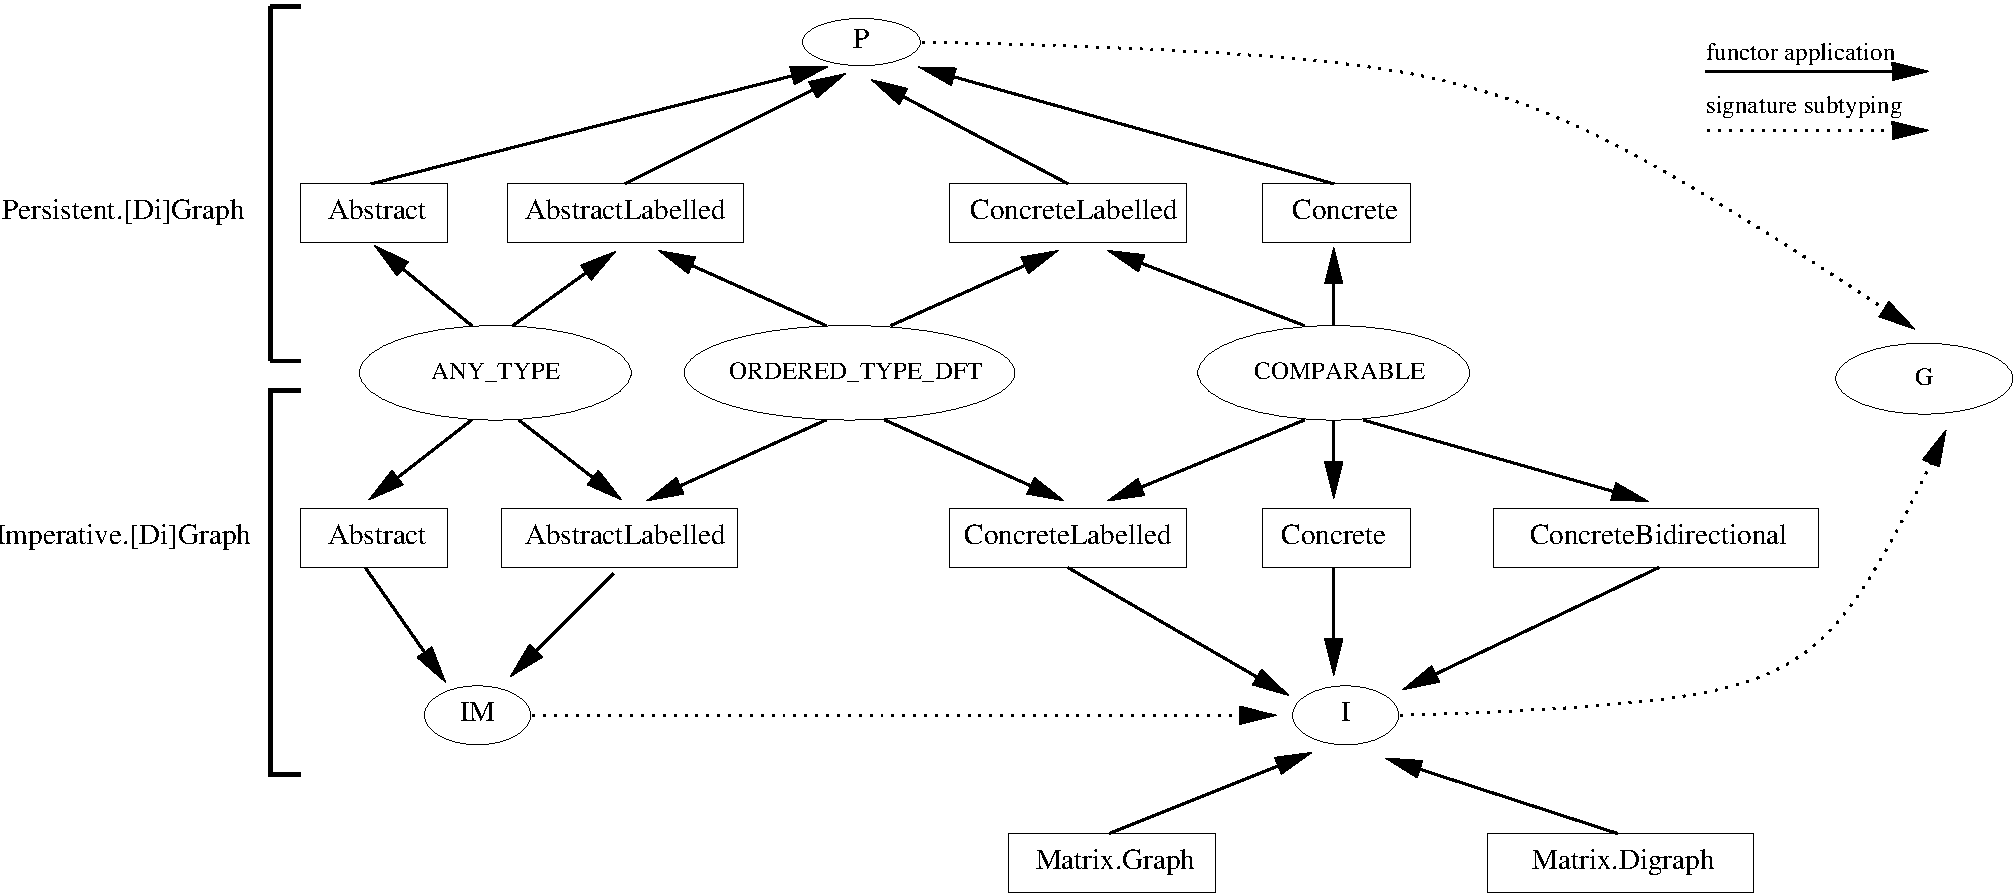
\includegraphics[width=\textwidth]{interface.pdf} 
\vskip-1pt
\begin{itemize}
\item 8 \bleu{persistent}: implemented with AVLs
\item 8 \bleu{imperative}: implemented with hash tables
\item 3 \bleu{specialized}: adjacency matrices and bidirectional graphs
\end{itemize}
\vskip-3pt
\begin{center}\emph{all together, 19 data structures}\end{center}
\end{frame}

\begin{frame}[fragile]
  \frametitle{Graph operations}
  \begin{itemize}
  \item \emph{creation} (insertion, suppression, etc.)
    \begin{alltt}
      val add_vertex : t \fleche\ vertex \fleche\ unit
    \end{alltt}
  \item \emph{test functions}
    \begin{alltt}
      val mem_edge : t \fleche\ vertex \fleche\ vertex \fleche\ bool
    \end{alltt}
  \item \emph{iterators} (vertices, edges, successors, etc.)
    \begin{alltt}
      val iter_vertex : (vertex \fleche\ unit) \fleche\ t \fleche\ unit
    \end{alltt}
  \end{itemize}
\end{frame}

\begin{frame}
  \frametitle{Graph algorithms}

  \begin{center}
    written independently of the graph implementation\\[1.2em]
    \emph{algorithm = functor}\\[1em]
  \end{center}
\end{frame}

\begin{frame}[fragile]
  \frametitle{Example: Shortest Path}

  \begin{enumerate}
  \item \emph{instantiating} the functor
  \begin{alltt}
    module W = struct
      type t = int
      let zero = 0
      let add = (+)
      ...
    end
    module Dij = \emph{Path.Dijkstra}(G)(W)
  \end{alltt}

  \item \emph{using} the resulting module
  \begin{alltt}
    let path,w = \emph{Dij.shortest_path} g v1 v2
  \end{alltt}
  \end{enumerate}
\end{frame}

\begin{frame}[fragile]
  \frametitle{Minimal Functor Signature}
only the \emph{required operations} as functor parameters
  \begin{alltt}
module type G = sig
  type t 
  module V : sig type t ... end
  module E : sig type t ... end
  val \emph{iter_succ_e} : (E.t -> unit) -> t -> V.t -> unit
end
module Dijkstra
  (G: G)
  (W: sig type t val \emph{weight} : G.E.t -> t ... end)
sig
  val shortest_path : G.t -> G.V.t -> G.V.t -> 
                      G.E.t list * W.t
end
  \end{alltt}
\end{frame}

\begin{frame}
  \frametitle{Benefits of functorized algorithms}

  \begin{itemize}
  \item clearly \emph{separates} algorithm from data structure\vskip8pt
  \item possible use on \emph{non-\ocamlgraph} data structures\vskip8pt
  \item easy \emph{extension} with new algorithms\vskip8pt
  \end{itemize}

\end{frame}

\begin{frame}
  \frametitle{Existing algorithms}
  \begin{itemize}
  \item traversal: 7 DFS, 2 BFS, 2 cycle detections
  \item building:
    \begin{itemize}
    \item classic graphs (e.g. de Bruijn's)
    \item random graphs (e.g. planar graph) 
    \end{itemize}
  \item Dijkstra's shortest path
  \item strongly connected components
  \item Goldberg's and Ford-Fulkerson's maximal flow
  \item $k$-coloring
  \item topological sorting
  \item Kruskal's minimum spanning tree
  \item misc. operations: transitive closure, complement, mirror,
    neighborhood, \dots
  \item interfaces with Graphviz and GML
\end{itemize}
\end{frame}

%%%%%%%%%%%%%%%%%%%%%%%%%%%%%%%%%%%%%%%%%%%%%%%%%%%%%%%%%%%%%%%%%%%%%%%%%%%%%%%

%\section[Implementation]{}

\begin{frame}
  \frametitle{Outline}
  \begin{itemize}
  \item \textcolor{black!30}{Using OcamlGraph\vskip15pt}
  \item Implementing OcamlGraph\vskip15pt
  \item \textcolor{black!30}{Conclusion\vskip15pt}
  \end{itemize}
\end{frame}

\begin{frame}
  \frametitle{Software Engineering}
  \begin{center}
    \bleu{How to code and to maintain 19 implementations \\ 
      and so many algorithms without difficulty?}
  \end{center}
\end{frame}

\begin{frame}
  \frametitle{Factorizing Code with Functors}
  \begin{enumerate}
  \item 
    abstracting the underlying implementation (AVL or hash table) by using a
    common signature \excode{HM}

  \vskip8pt\pause
  \item 
    one functor for each feature
    \vskip1pt
    \begin{itemize}
    \item \excode{Minimal}: common operations
      \vskip6pt
    \item \excode{Labeled}/\excode{Unlabeled}
      \vskip6pt
    \item \excode{Pred}: predecessors from successors
      \vskip6pt
    \item \excode{Make\_Abstract}: abstract graphs from concrete ones
    \end{itemize}
  \end{enumerate}
\end{frame}

\begin{frame}[containsverbatim]
  \frametitle{Example}

persistent or imperative unlabeled directed graphs

\begin{alltt}
\motcle{module} Make
  (F: \motcle{functor}(X: COMPARABLE) \fleche HM \motcle{with type} key = X.t) = 
\motcle{struct}
  \motcle{module} Digraph = \motcle{struct}
    \motcle{module} Concrete(V: COMPARABLE) = \motcle{struct}
      \motcle{include} \emph{ConcreteVertex}(F)(V)
      \motcle{include} \emph{Unlabeled}(V)(HM)
      \motcle{include} \emph{Minimal}(S)(HM)
    \motcle{end}
\motcle{end}
\motcle{module} I = Make(Make_Hashtbl)
\motcle{module} P = Make(Make_Map)
\end{alltt}
\end{frame}

\begin{frame}
  \frametitle{Code Factorization}

  \begin{center}
    all together, 19 data structures with 45 operations each \\[1em]
    
    \emph{855 operations in 1000 lines of code}
  \end{center}
\end{frame}


%%%%%%%%%%%%%%%%%%%%%%%%%%%%%%%%%%%%%%%%%%%%%%%%%%%%%%%%%%%%%%%%%%%%%%%%%%%%%%%


\begin{frame}
  \frametitle{Outline}
  \begin{itemize}
    \item \textcolor{black!30}{Using OcamlGraph\vskip15pt
    \item Implementing OcamlGraph\vskip15pt}
  \item Conclusion
  \end{itemize}
\end{frame}

\begin{frame}
  \frametitle{Comparison}
  \begin{center}
  \begin{tabular}{|l||c|c|c|c|c|}
    \hline
     Library & Language     &P/I& Genericity & Data struct. \\\hline\hline
     GTL & C++     & I & \absent  & 1  \\\hline
     LEDA & C++    & I & \absent  & 2  \\\hline
     BGL & C++     & I & \present & 2  \\\hline
     JDSL & Java   & I & \present & 1  \\\hline
     FGL & Haskell & P & \absent  & 1  \\\hline
     MLRisc & SML  & I & \absent  & 1  \\\hline
%     Baire & Ocaml &P/I& ---      & 8  \\\hline
     \emph{\ocamlgraph}& Ocaml &P/I& \present & \emph{19} \\\hline
  \end{tabular}
  \end{center}
\end{frame}

\begin{frame}
  \frametitle{Figures}
  \begin{itemize}
  \item \ocamlgraph\ is\vskip2pt
    \begin{itemize}
    \item 7000 lines of code (2000 lines of external contributions)
      \vskip7pt
    \item 9 men-weeks of work
    \end{itemize}
    \begin{center}
      \emph{only possible thanks to ML functors}
    \end{center}\vskip10pt
    \pause
  \item benchmarks\vskip2pt
    \begin{itemize}
    \item creation rate $\approx$ 100 000 edges per second\vskip7pt
    \item traversal rate $\approx$ 1 million edges per second
    \end{itemize}
    \begin{center}
      \emph{compares to other graph libraries}
    \end{center}
  \end{itemize}
\end{frame}

%%%%%%%%%%%%%%%%%%%%%%%%%%%%%%%%%%%%%%%%%%%%%%%%%%%%%%%%%%%%%%%%%%%%%%%%%%%%%%%

\end{document}
    
